\section{The Parallel Algorithm}
\label{sec:parallel-algorithm}

In this section, we detail the data structures and algorithms used in the parallel implementation of the quadtree-adaptive HPS method. We start by going over the leaf-indexed quadtree provided from \pforest\ and the path-indexed quadtree. This leads into how these data structures are implemented in parallel, including communication patterns. Finally, this leads to a discussion of the merging and splitting algorithms in parallel.

\subsection{MPI Preliminaries}

We define and assume the following with regard to using the Message Passing Interface (MPI) \citep{mpi40}. A {\em rank} is a compute unit with a separate, unique memory space. Each rank in the execution of a program runs a separate version of the program. {\em Communication} is how data is shared via {\em messages} between ranks and is associated with actions such as sending, receiving, or broadcasting messages. A {\em communicator} is a union of ranks in which each rank has a unique index $R_i = 0, ..., N_{R}-1$, where $N_R$ is the number of ranks in a communicator. In every MPI program, there is a global communicator called {\tt MPI\_COMM\_WORLD} that contains all ranks that are executing the program.

\subsection{Quadtree Data Structures}
\label{sub:quadtree-data-structures}

\begin{figure}
    \centering
    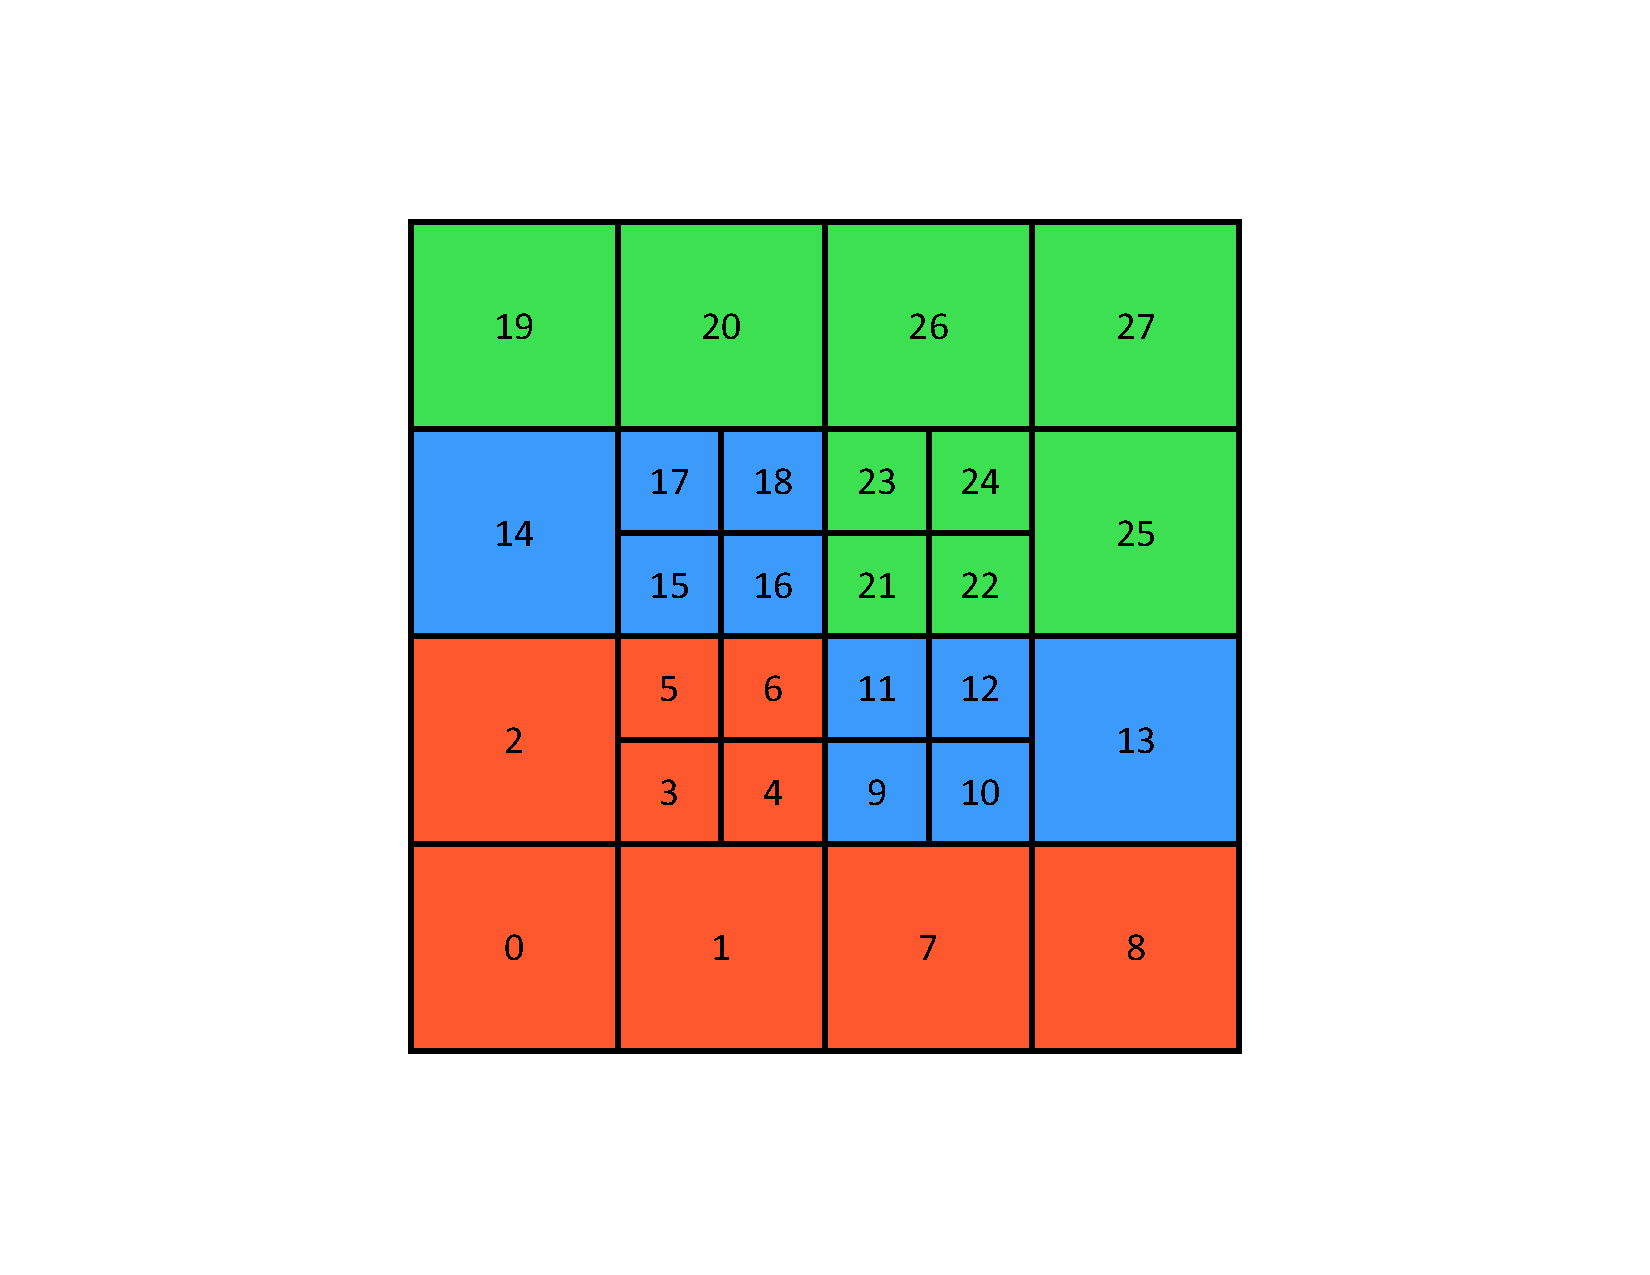
\includegraphics[width=\textwidth, clip=true, trim={0 100 0 100}]{figures/parallel_adaptive_mesh_indexing.pdf}
    \caption{An example of an adaptive, quadtree mesh that is refined around the center of the domain. The colors denote different ranks and the numbers indicate the leaf-index of the quadrant.}
    \label{fig:adaptive_mesh}
\end{figure}

\begin{figure}
    \centering
    \begin{tabular}{c}
    \smallskip
        \begin{subfigure}[t]{0.8\textwidth}
            \centering
            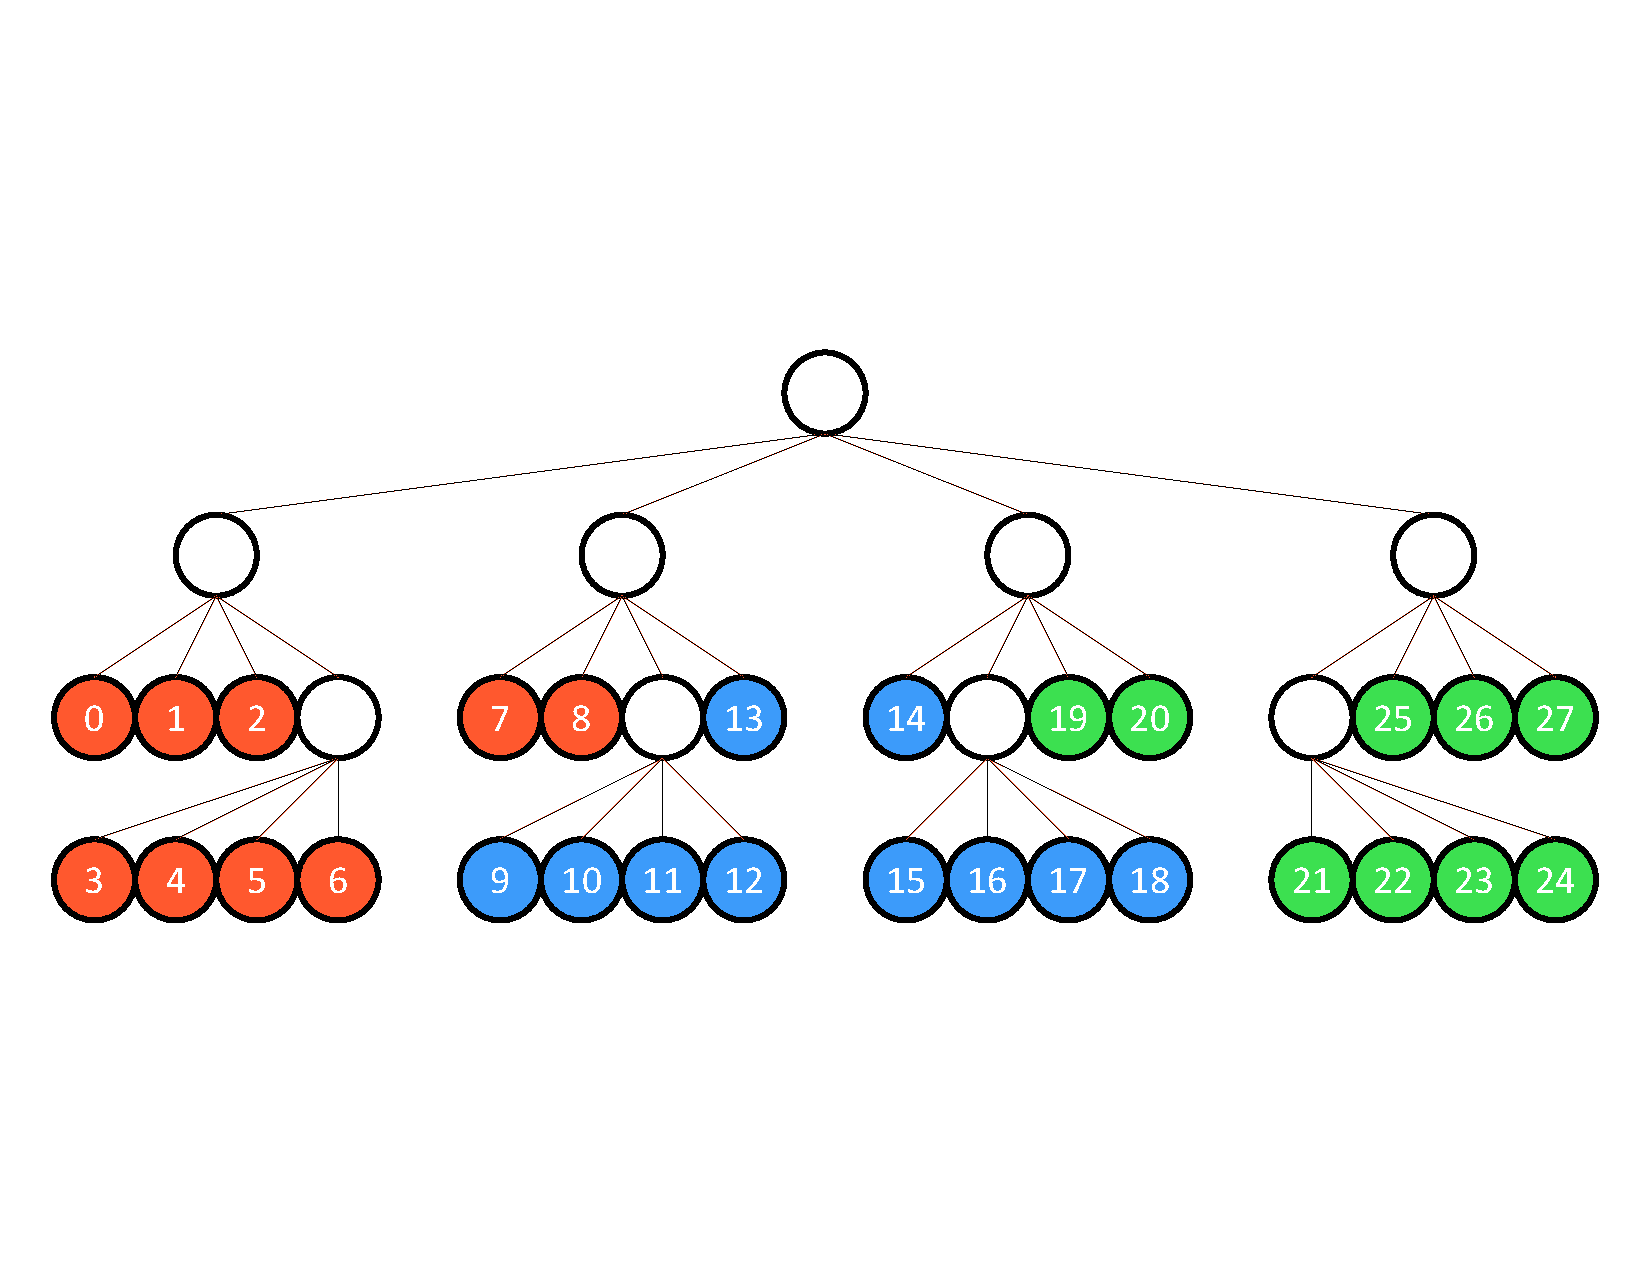
\includegraphics[width=\textwidth, clip=true, trim={0 150 0 150}]{figures/parallel_leaf_indexed_tree.pdf}
            \caption{Leaf-level indexing of quadtree nodes}
            \label{subfig:leaf-indexed-quadtree}
        \end{subfigure}
        \\
        \begin{subfigure}[t]{0.8\textwidth}
            \centering
            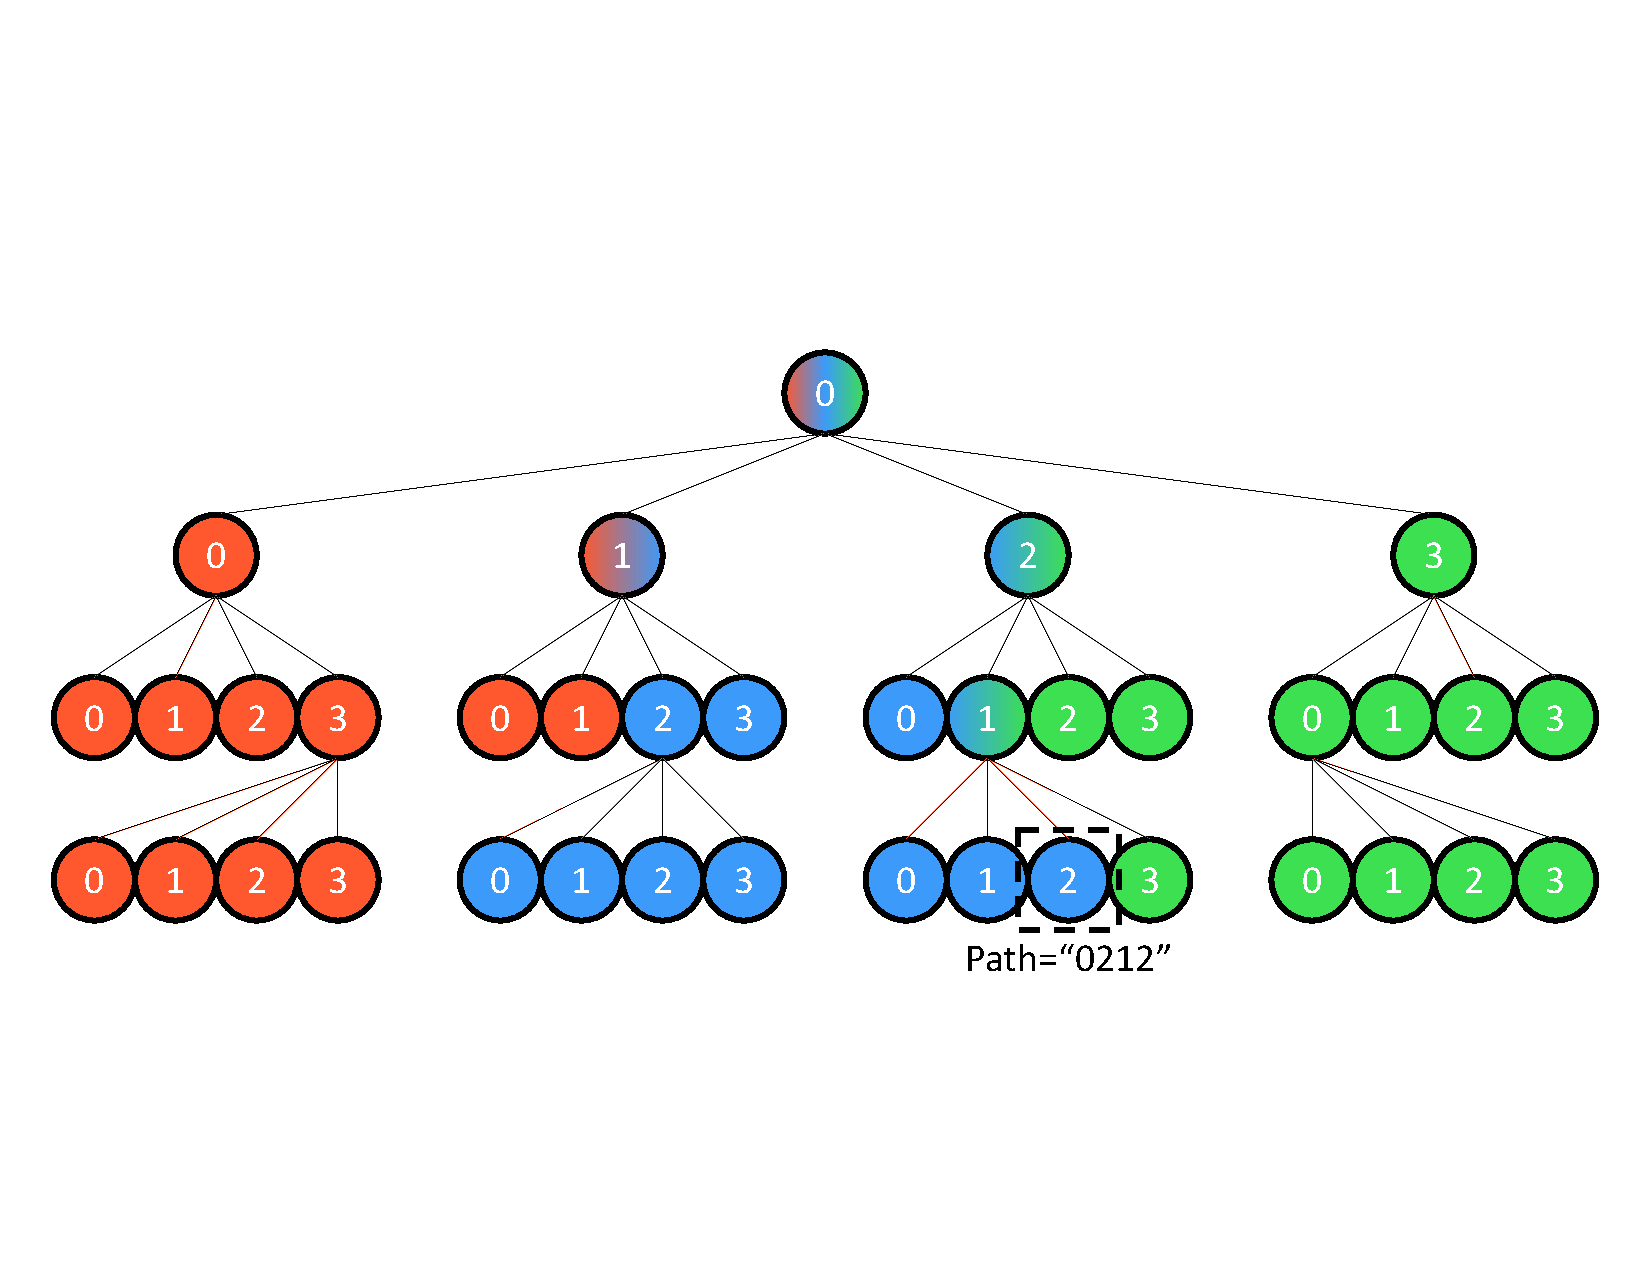
\includegraphics[width=\textwidth, clip=true, trim={0 140 0 150}]{figures/parallel_path_indexed_tree.pdf}
            \caption{Path indexing of quadtree nodes}
            \label{subfig:path-indexed-quadtree}
        \end{subfigure}
    \end{tabular}\\
    \caption{Leaf-indexed vs. path-indexed quadtrees. Both trees represent the mesh found in \reffig{fig:adaptive_mesh}. The colors denote which rank owns each node. In (a), only the leaves of a quadtree are indexed and stored. In (b), all nodes of the quadtree are indexed and stored according to their unique path. Note that the nodes in (b) that are colored with a gradient (i.e., ``0'', ``01'', ``02'', ``021'') are owned by multiple ranks.}
    \label{fig:quadtree_indexing}
\end{figure}

The \pforest\ library provides a leaf-indexed quadtree data structure and functions to construct, store, and iterate over leaf-level nodes (also called quadrants). The \pforest\ quadtree only stores leaf-level quadrants. Quadrants in a \pforest\ quadtree are stored locally to each rank, with minimal redundant metadata stored on each rank to handle the logic for where each quadrant is stored. The quadrants are stored in a rank-local linked list and indexed according to a space-filling curve. Partitioning in \pforest\ results in an equally-divided quadtree where each rank has roughly the same number of quadrants, subject to the integer division of the number of leaf-nodes $N_{L}$ into $N_{R}$.

As outlined in \citep{chipman2024fast}, the HPS method requires storage for all nodes in a quadtree, including leaves and ancestors. This is to store the set of matrices that act as the factorization of the system matrix. We developed a path-indexed quadtree that builds upon the quadtrees provided in \pforest\ and has storage for all nodes in the quadtree. The path-indexed quadtree indexes each node in the tree according to the path of the node, where a path is the unique series of directions required to traverse from the root of the tree to the node in question. Each node can be uniquely indexed according to its path. The path is used as a key in a key-value lookup table (i.e. map) to provide storage for each node in the path-indexed quadtree. \reffig{fig:quadtree_indexing} depicts the leaf-indexed and path-indexed quadtrees, including colors that denote which ranks own each node.

In parallel, the leaf nodes of a leaf-indexed quadtree are partitioned across available ranks. The partitioning of a path-indexed quadtree follows the partitioning of a leaf-indexed quadtree. Any node in a path-indexed quadtree has a range of ranks from \rfirst to \rlast on which that node exists. A leaf node is always local to a single rank, or \rfirst $=$ \rlast. The parents and ancestors of the leaf nodes can exist across multiple ranks depending on the range of ranks of a node's descendants. The range of ranks is provided from \pforest\ upon initialization of the path-indexed quadtree and associated nodes.

The range of ranks allows for creation of a {\em node communicator}. A node communicator is a subset of the global communicator that includes only the range of ranks a particular node lives on. When communication is necessary (as in the 4-to-1 merge or the 1-to-4 split algorithms), a node may communicate its data to all ranks that store a version of that node in the quadtree. Creation of the node communicator is a collective routine on all ranks that are part of the super communicator. The node communicators are created and stored on each node during the initialization of the path-indexed quadtree to avoid global communication when performing the factorization or solves.

Initialization of a path-indexed quadtree assumes a leaf-indexed quadtree already exists. The leaf-indexed quadtree (a \pforest\ object) can be created by refining a quadrant according to a refinement criteria that is problem dependent (see \reffig{fig:adaptive_mesh}). The leaf-indexed quadtree is not required to have data associated with each quadrant, so there is minimal redundant logical storage. Once a leaf-indexed quadtree is refined, the path-indexed quadtree can be created through a depth-first traversal of the leaf-indexed quadtree. This utility is provided in the \codename{p4est\_search\_all} function.

The callback function provided to \codename{p4est\_search\_all} is found in \refalg{alg:p4est_search_all_callback}. \pforest\ also provides a utility to get the index of a quadrant's ancestor in \codename{p4est\_quadrant\_ancestor\_id}. This function is used to create the path of the quadrant (represented as a string) that is used as the key in the map that stores the nodes in the path-indexed quadtree. The main idea of \refalg{alg:p4est_search_all_callback} is to allocate space in the map if the rank executing the code owns the node in the quadtree, and if not, set that space in the map to \codename{nullptr}. The node is created either from the root data (provided from the user) or the parent data. In practice, a factory design pattern is used to generate the nodes; the user implements a node factory object.

\begin{algorithm}
    \caption{\codename{p4est\_search\_all\_callback} Function}
    \begin{algorithmic}[0]
        \Require $\mathcal{Q}_{L}$, $\mathcal{Q}_{P}$, $\Omega_i$, $R_{\text{first}}$, $R_{\text{last}}$
        \State Get \codename{map} from $\mathcal{Q}_{P}$
        \State Compute \codename{path} from \codename{p4est\_quadrant\_ancestor\_id}($\Omega_i$)
        \State Let \codename{owned} = $R_{\text{first}} < r < R_{\text{last}}$
        \If {\codename{owned}}
            \If {$\Omega_i$ is the root quadrant}
                \State Create \codename{node\_ptr} from root data: \codename{node\_ptr} $\rightarrow \Omega^{\tau}$
            \Else
                \State Create \codename{node\_ptr} from parent data: \codename{node\_ptr} $\rightarrow \Omega^{\tau}$
            \EndIf
            \State Let \codename{map[path] = node\_ptr}
        \Else
            \State Let \codename{map[path] = nullptr}
        \EndIf
    \end{algorithmic}
    \label{alg:p4est_search_all_callback}
\end{algorithm}

The merging and splitting algorithms detailed in \refsec{sub:stages-of-the-quadtree-adaptive-hps-method} require references to the data stored on the parent node and the children nodes associated with the merge or split. When children nodes are not rank-local, communication is necessary to share the data across ranks. Ranks within a node communicator broadcast their associated data to other involved ranks to ensure that each rank has a local copy of all children and parent nodes. For example, from \reffig{fig:quadtree_indexing}(b), when merging children nodes ``0210'', ``0211'', ``0212'', and ``0213'' into parent node ``021'', the yellow rank must broadcast nodes ``0210'', ``0211'', and ``0212'' to the green rank, and the green rank must broadcast node ``0213'' to the yellow rank. Both yellow and green ranks would already have storage for the parent node ``021''.

The algorithm for communicating families of nodes among ranks is outlined in \refalg{alg:p4est_search_merge_split}. This is the function that is passed to \codename{p4est\_search\_reorder} either for the pre-quadrant callback (splitting algorithms) or the post-quadrant callback (merging algorithms). The primary logic of \refalg{alg:p4est_search_merge_split} checks if the node is a leaf or not to call either \codename{LeafCallback} or \codename{FamilyCallback} and if the node is local to the rank executing this code. In order to call \codename{MPI\_Bcast}, the root rank must be known. This is the rank that sends the data in the broadcast; all other nodes receive the data and store it in a rank-local buffer. A call to \codename{MPI\_Allreduce} for each children node communicates which rank is the root rank for that node. The call to \codename{MPI\_Bcast} provides the buffer for ranks to send and receive node data and only communicates within the node communicator.

\begin{algorithm}
    \caption{\codename{p4est\_search\_merge\_split} Function}
    \begin{algorithmic}[0]
        \Require $\mathcal{Q}_{L}$, $\mathcal{Q}_{P}$, $\Omega_i$, $R_{\text{first}}$, $R_{\text{last}}$
        \State Get \codename{map} from $\mathcal{Q}_{P}$
        \State Compute \codename{path} from \codename{p4est\_quadrant\_ancestor\_id}($\Omega_i$)
        \State Let \codename{node\_ptr} = \codename{map[path]}: \codename{node\_ptr} $\rightarrow \Omega^{\tau}$
        \State Let \codename{owned} = $R_{\text{first}} < r < R_{\text{last}}$
        \State Let \codename{children\_ptrs} = $\{\}$
        \If{$i$ $\ge$ 0 $\And$ \codename{node\_ptr} $\ne$ \codename{nullptr} $\And$ \codename{owned}}
            \State Call \codename{LeafCallback(node\_ptr)}
        \Else
            \If{$R_{\text{first}} = R_{\text{last}}$}
                \For{$i = 0, ..., 3$}
                    \State Let \codename{children\_ptrs[i] = map[path + string(i)]}
                \EndFor
            \ElseIf{\codename{owned}}
                \For{$i = 0, ..., 3$}
                    \State Let \codename{child\_ptr = map[path + string(i)]}
                    \State Communicate \codename{child\_ptr} to all ranks in \codename{node\_comm}
                    \State Let \codename{children\_ptrs[i] = child\_ptr}
                \EndFor
            \EndIf
            \If{\codename{owned}}
                \State Call \codename{FamilyCallback(node\_ptr, children\_ptrs)}
            \EndIf
        \EndIf
    \end{algorithmic}
    \label{alg:p4est_search_merge_split}
\end{algorithm}